\documentclass[11pt]{article}
\usepackage[margin=1in]{geometry}
\usepackage{amsmath,amssymb}
\usepackage{booktabs}
\usepackage{graphicx}
\usepackage{hyperref}
\usepackage{microtype}
\title{Transient Low-Order Cues Bootstrap High-Order Compositional Representations in Transformers}
\author{Project Kepler Collaboration}
\date{}
\begin{document}
\maketitle

\begin{abstract}
We study whether training-distribution geometry can alter formation of a
high-order predictive representation while the target conditional,
irreducible noise, marginals, and total predictable information remain fixed.
In a finite-field parent-exposed task, two uniform parents determine a modular
center and a fixed additive-noise channel determines the target. Version 3.5
provided exploratory evidence that transient full-support low-order cues
advanced predictive-state formation. An independent v3.6 replication used two
new rules, two new cue permutations, two initialization seeds, and three cue
doses. Verified onset occurred in 1/8,
6/8, and 8/8 blocks. The frozen
one-sided exact blocked Page-style test enumerated
1,679,616 assignments and gave
$p=9.5259869e-06$. All 13 nonzero-cue cells
positive at cue removal retained the representation threshold at 6M and 10M.
Temporary cue-bearing distributions therefore causally changed onset timing or
probability within the frozen task and model family. The experiment does not
identify singleton mutual information alone as causal and does not establish a
universal Transformer property.
\end{abstract}

\section{Introduction}
The central question is: \emph{How does training-distribution geometry affect
the accessibility of task-sufficient representations when the final task
information is fixed?} A representation may be statistically available yet
difficult to discover because useful optimization directions are weak, cancel
across examples, or become accessible only after other features organize. We
therefore intervene on early training-distribution geometry while holding the
target conditional and information budget fixed.

Project Kepler uses a finite-field mechanism assay motivated by, but distinct
from, its recurrent production task. The parent-exposed design intentionally
separates (1) identifying relevant variables, which the interface controls by
presenting both parents directly, from (2) composing discovered variables into
a predictive representation, which remains the learning problem. The present
paper does not claim that the recurrent task has been solved.

Version 3.5 is exploratory discovery; version 3.6 is an independent
confirmatory replication. The discovery data are excluded from the primary
confirmatory $p$-value. The aim is neither a new scaling law nor a universal
intelligence principle; it is a bounded causal test within one controlled task
and model family. Figure~\ref{fig:task} summarizes the construction and cue
schedule.

\begin{figure}[tb]
\centering
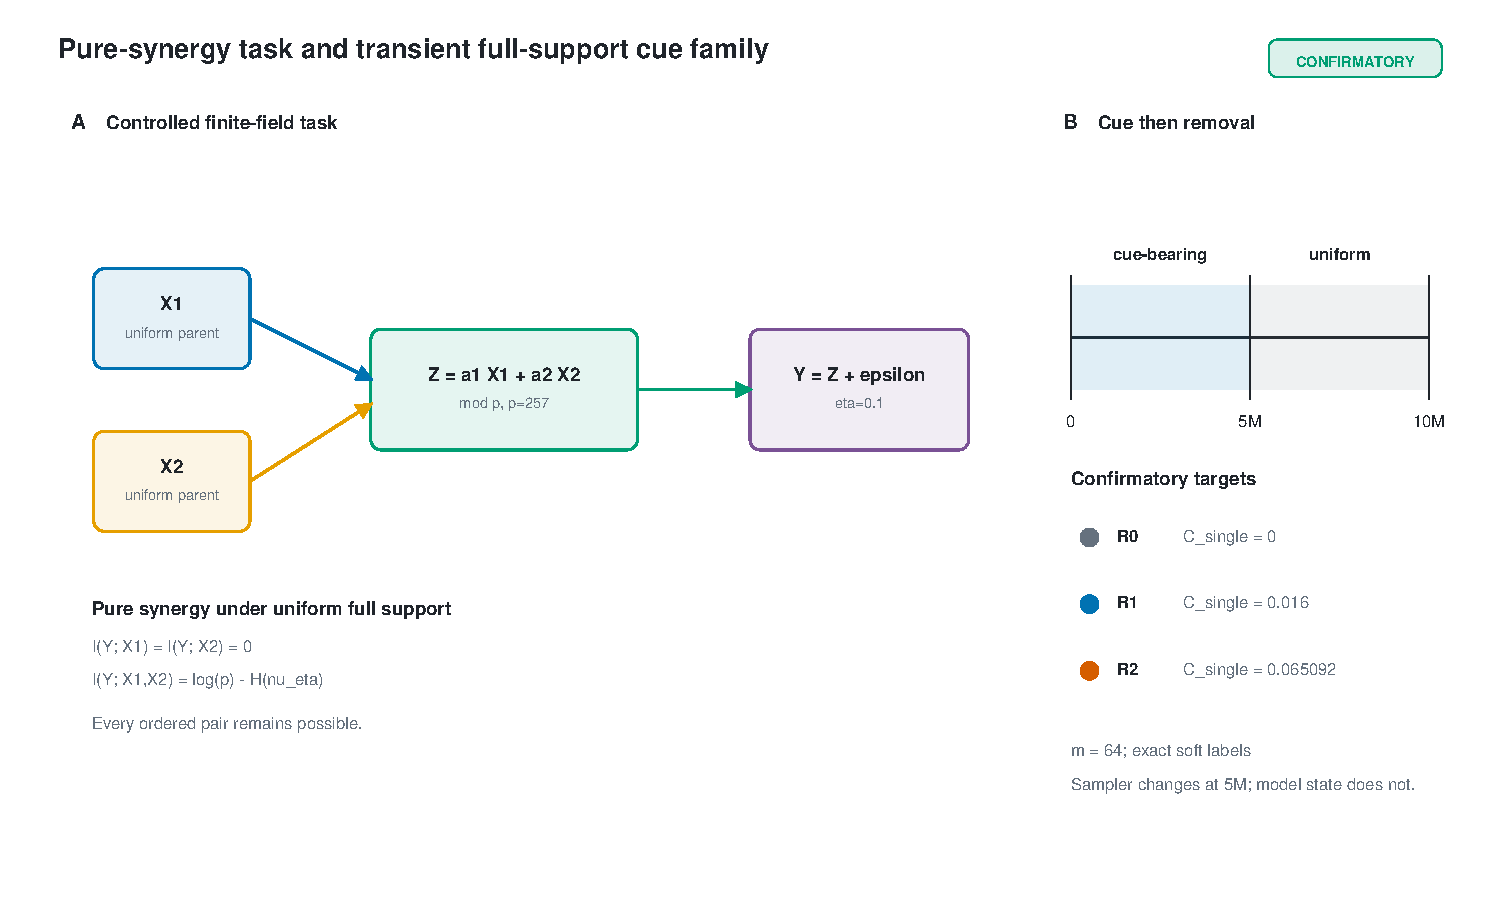
\includegraphics[width=\linewidth]{figures/fig01_task_cue_schematic.pdf}
\caption{Controlled finite-field task and transient cue schedule. All values
are generated from frozen JSON.}
\label{fig:task}
\end{figure}

\section{Related Work}
\paragraph{Grokking and delayed generalization.}
Modular-arithmetic grokking studies established that small neural networks can
generalize long after achieving near-perfect training performance under a
fixed training distribution \cite{power2022grokking}. This paper does not
offer a universal explanation of grokking. It instead asks whether the
geometry of the \emph{early} training distribution, with the final
conditional and information budget held fixed, changes the accessibility or
timing of a delayed representational transition.

\paragraph{Mechanistic interpretability of modular arithmetic.}
Mechanistic analyses of modular addition have recovered Fourier-like internal
representations and circuits implementing trigonometric structure
\cite{nanda2023progress}. Here, fixed-Fourier probes are diagnostics
alongside linear and fixed-capacity MLP probes. We do not assume that a
specific Fourier circuit must be learned, and the causal result concerns the
timing or probability of task-sufficient representation formation rather than
identification of a unique circuit.

\paragraph{Curriculum learning.}
Classic curriculum learning changes example order or introduces examples and
concepts by increasing difficulty \cite{bengio2009curriculum}. The present
intervention instead keeps the target conditional and Bayes information
budget fixed and changes only the geometry of the full-support training
distribution during an early window. We call this narrower intervention
\emph{distributional bootstrapping of representation formation}.

\paragraph{Partial Information Decomposition.}
Partial Information Decomposition separates redundant, unique, and
synergistic contributions in multivariate information
\cite{williams2010pid}. The full-support base task is a pure-synergy
construction in the limited operational sense needed here: singleton
information is zero while joint information is nonzero. We do not attempt a
full PID decomposition of the cue distributions or learned representations.

\section{Controlled finite-field task}
The field size is $p=257$. The predictive center is
$z=a_1x_1+a_2x_2 \bmod p$, and $y=z+\epsilon \bmod p$ with
$P(\epsilon=0)=1-\eta$, $P(\epsilon=r)=\eta/(p-1)$ for $r\ne0$, and
$\eta=0.1$. Thus $H(Y\mid X_1,X_2)=0.879601$ nats, and the
target conditional is unchanged across conditions. The primary metric is
\[
R=\frac{\mathbb{E}_h D_{\rm KL}(q_h\Vert p_\theta)}
{\log p-H(\nu_\eta)}.
\]
A uniform predictor has $R=1$ and the oracle has $R=0$. Objective,
evaluation, bootstrap, and probe details appear in Supplementary Methods.

\section{Pure-synergy information structure}
Under uniform full support, $X_1,X_2,Z,Y$ are uniform,
$I(Y;X_1)=I(Y;X_2)=0$, and
$I(Y;X_1,X_2)=4.66948$ nats. The scalar cue index orders
selected constructed distributions; it is not a unique-information percentage.

\section{Full-support cue-family construction}
The cue family reweights ordered parent pairs through frozen permutations while
retaining strictly positive support. Exhaustive enumeration verifies uniform
marginals, invariant $H(Y\mid X_1,X_2)$, invariant joint information, and exact
uniform full support at zero cue. The intervention is the registered
distribution, not singleton mutual information in isolation.
Table~\ref{tab:table01-distribution-invariants} reports the frozen audits;
construction details appear in Supplementary Methods.

\begin{table}[tb]
\centering
\caption{Every registered cue distribution retained strict full support and the frozen information identities.}
\label{tab:table01-distribution-invariants}
\resizebox{\linewidth}{!}{%
\begin{tabular}{lrrrrrrrrrrrrr}
\toprule
Version & Status & Rule & Permutation & Condition & m & Target C\_single & Achieved C\_single & Lambda & Min pair probability & Max uniformity error & H(Y|X1,X2), nats & Joint-I abs. error & Strict support \\
\midrule
v3.5 & exploratory & 45,36 & v3.5 & C0 & 64 & 0 & 7.608e-16 & 0 & 1.514e-05 & 9.107e-18 & 0.879601 & 1.066e-14 & yes \\
v3.5 & exploratory & 45,36 & v3.5 & C1 & 64 & 0.016 & 0.016 & 0.182955 & 1.237e-05 & 2.602e-18 & 0.879601 & 0 & yes \\
v3.5 & exploratory & 45,36 & v3.5 & C2 & 64 & 0.065092 & 0.065092 & 0.38055 & 9.379e-06 & 1.735e-18 & 0.879601 & 1.776e-15 & yes \\
v3.5 & exploratory & 45,36 & v3.5 & C3 & 64 & 0.13 & 0.13 & 0.546166 & 6.871e-06 & 9.107e-18 & 0.879601 & 5.329e-15 & yes \\
v3.5 & exploratory & 45,36 & v3.5 & geometry\_concentrated & 1 & 0.065092 & 0.065092 & 0.078826 & 1.395e-05 & 1.908e-17 & 0.879601 & 1.599e-14 & yes \\
v3.5 & exploratory & 45,36 & v3.5 & geometry\_diffuse & 128 & 0.065092 & 0.065092 & 0.594889 & 6.133e-06 & 5.638e-18 & 0.879601 & 1.776e-15 & yes \\
v3.6 & confirmatory & 205,5 & permutation\_0 & R0 & 64 & 0 & 7.608e-16 & 0 & 1.514e-05 & 9.107e-18 & 0.879601 & 1.066e-14 & yes \\
v3.6 & confirmatory & 205,5 & permutation\_0 & R1 & 64 & 0.016 & 0.016 & 0.182955 & 1.237e-05 & 1.735e-18 & 0.879601 & 0 & yes \\
v3.6 & confirmatory & 205,5 & permutation\_0 & R2 & 64 & 0.065092 & 0.065092 & 0.38055 & 9.379e-06 & 1.301e-18 & 0.879601 & 0 & yes \\
v3.6 & confirmatory & 205,5 & permutation\_1 & R0 & 64 & 0 & 7.608e-16 & 0 & 1.514e-05 & 9.107e-18 & 0.879601 & 1.066e-14 & yes \\
v3.6 & confirmatory & 205,5 & permutation\_1 & R1 & 64 & 0.016 & 0.016 & 0.182955 & 1.237e-05 & 1.735e-18 & 0.879601 & 0 & yes \\
v3.6 & confirmatory & 205,5 & permutation\_1 & R2 & 64 & 0.065092 & 0.065092 & 0.38055 & 9.379e-06 & 1.301e-18 & 0.879601 & 0 & yes \\
v3.6 & confirmatory & 123,209 & permutation\_0 & R0 & 64 & 0 & 7.608e-16 & 0 & 1.514e-05 & 9.107e-18 & 0.879601 & 1.066e-14 & yes \\
v3.6 & confirmatory & 123,209 & permutation\_0 & R1 & 64 & 0.016 & 0.016 & 0.182955 & 1.237e-05 & 1.735e-18 & 0.879601 & 0 & yes \\
v3.6 & confirmatory & 123,209 & permutation\_0 & R2 & 64 & 0.065092 & 0.065092 & 0.38055 & 9.379e-06 & 1.301e-18 & 0.879601 & 0 & yes \\
v3.6 & confirmatory & 123,209 & permutation\_1 & R0 & 64 & 0 & 7.608e-16 & 0 & 1.514e-05 & 9.107e-18 & 0.879601 & 1.066e-14 & yes \\
v3.6 & confirmatory & 123,209 & permutation\_1 & R1 & 64 & 0.016 & 0.016 & 0.182955 & 1.237e-05 & 2.602e-18 & 0.879601 & 0 & yes \\
v3.6 & confirmatory & 123,209 & permutation\_1 & R2 & 64 & 0.065092 & 0.065092 & 0.38055 & 9.379e-06 & 1.301e-18 & 0.879601 & 0 & yes \\
\bottomrule
\end{tabular}%
}
\end{table}


\section{Exploratory discovery experiment}
Version 3.5 used rule $(45,36)$, five paired seeds, four ordered $m=64$ doses,
and two matched-index geometry controls. Verified onset occurred in
0/5 C0, 5/5 C1, 5/5 C2, and
5/5 C3 seeds. The exploratory exact test gave
$p=1.6075103e-05$. These observations selected frozen
confirmatory conditions and definitions; they are not confirmatory data.

\begin{figure}[tb]
\centering
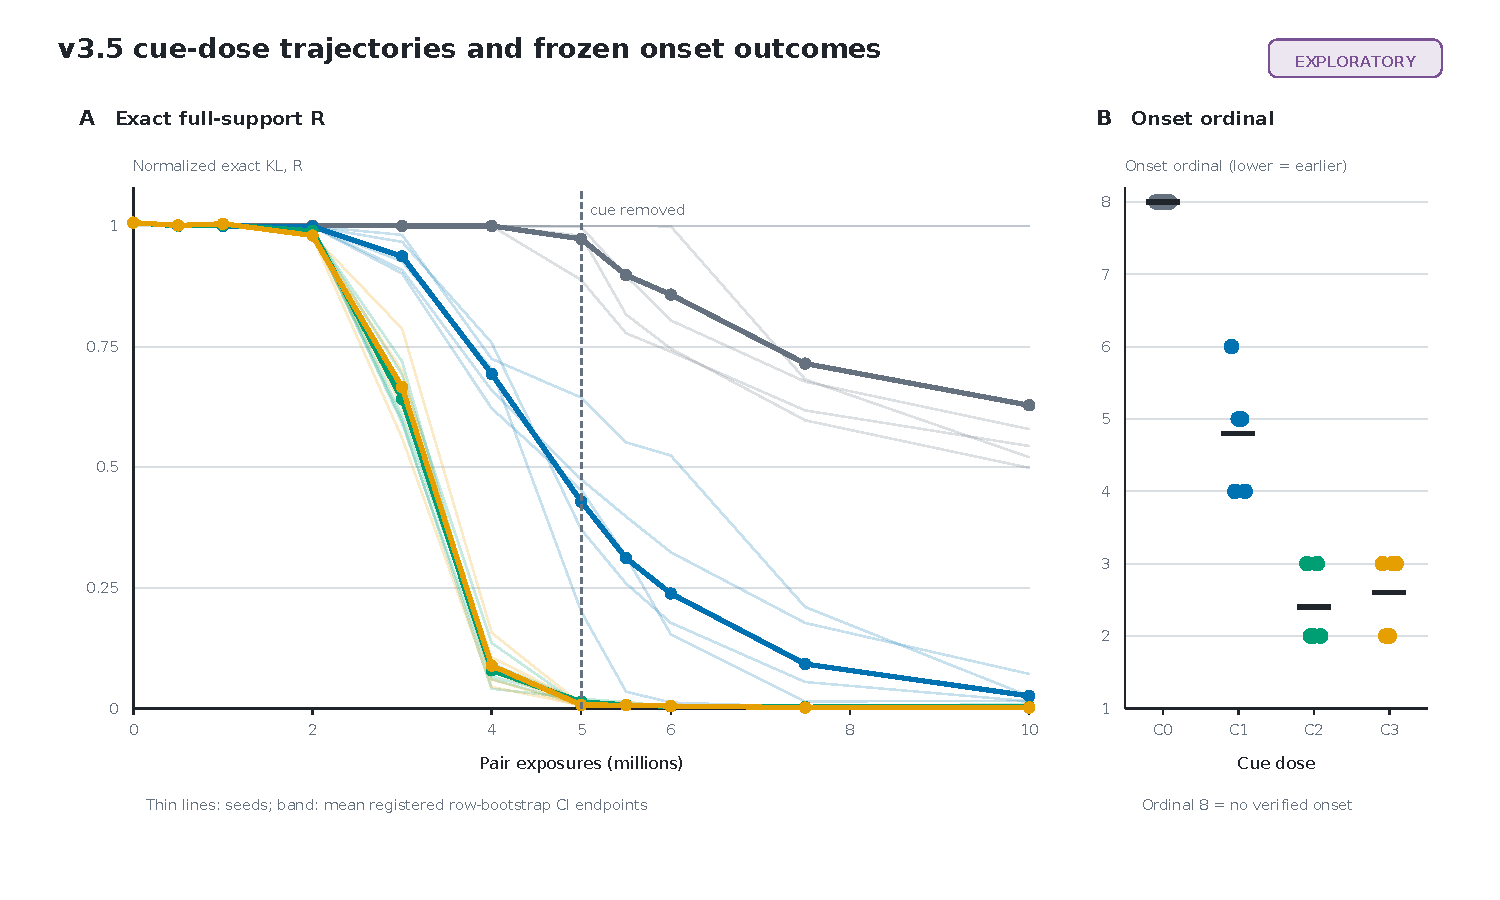
\includegraphics[width=\linewidth]{figures/fig02_v35_dose_trajectories.pdf}
\caption{Exploratory v3.5 R trajectories and onset outcomes. Bands are means
of registered row-bootstrap endpoints, not new group-level intervals.}
\label{fig:v35-trajectories}
\end{figure}

\begin{table}[!htbp]
\centering
\caption{Exploratory discovery outcomes decoded with the frozen onset and establishment rules.}
\label{tab:table02-v35-exploratory-outcomes}
\resizebox{\linewidth}{!}{%
\begin{tabular}{lrrrrrrrrrrr}
\toprule
Version & Status & Condition & n & Onset by 5M & Onset by 10M & Onset exposures (M) & Terminal ordinals & Established by 5M & Established by 10M & Mean R, 5M pre & Mean R, 10M \\
\midrule
v3.5 & exploratory & C0 & 5 & 0 & 0 & —, —, —, —, — & 8, 8, 8, 8, 8 & 0 & 0 & 0.973341 & 0.628411 \\
v3.5 & exploratory & C1 & 5 & 2 & 5 & 7.5, 5, 6, 6, 5 & 6, 4, 5, 5, 4 & 0 & 5 & 0.428643 & 0.025721 \\
v3.5 & exploratory & C2 & 5 & 5 & 5 & 4, 3, 3, 4, 3 & 3, 2, 2, 3, 2 & 5 & 5 & 0.013564 & 0.003252 \\
v3.5 & exploratory & C3 & 5 & 5 & 5 & 4, 3, 3, 4, 4 & 3, 2, 2, 3, 3 & 5 & 5 & 0.007108 & 0.00162 \\
v3.5 & exploratory & geometry\_concentrated & 5 & 5 & 5 & 4, 5, 4, 5, 4 & 3, 4, 3, 4, 3 & 5 & 5 & 0.014501 & 0.001528 \\
v3.5 & exploratory & geometry\_diffuse & 5 & 5 & 5 & 5, 3, 3, 3, 4 & 4, 2, 2, 2, 3 & 4 & 5 & 0.055923 & 0.007754 \\
\bottomrule
\end{tabular}%
}
\end{table}

Figure~\ref{fig:v35-trajectories} and
Table~\ref{tab:table02-v35-exploratory-outcomes} report the discovery
trajectories and frozen outcomes.

\section{Independent confirmatory replication}
Version 3.6 crossed two new rules with two new cue permutations and two new
initialization seeds, yielding eight paired blocks and 24 trajectories. R0,
R1, and R2 shared initial weights and all non-condition random fields within
each block. Verified onset occurred in 1/8,
6/8, and 8/8 blocks. The observed
Page-style statistic was 110.0; exactly
16 of 1,679,616
assignments were as large, giving one-sided
$p=9.5259869e-06$.

\begin{figure}[tb]
\centering
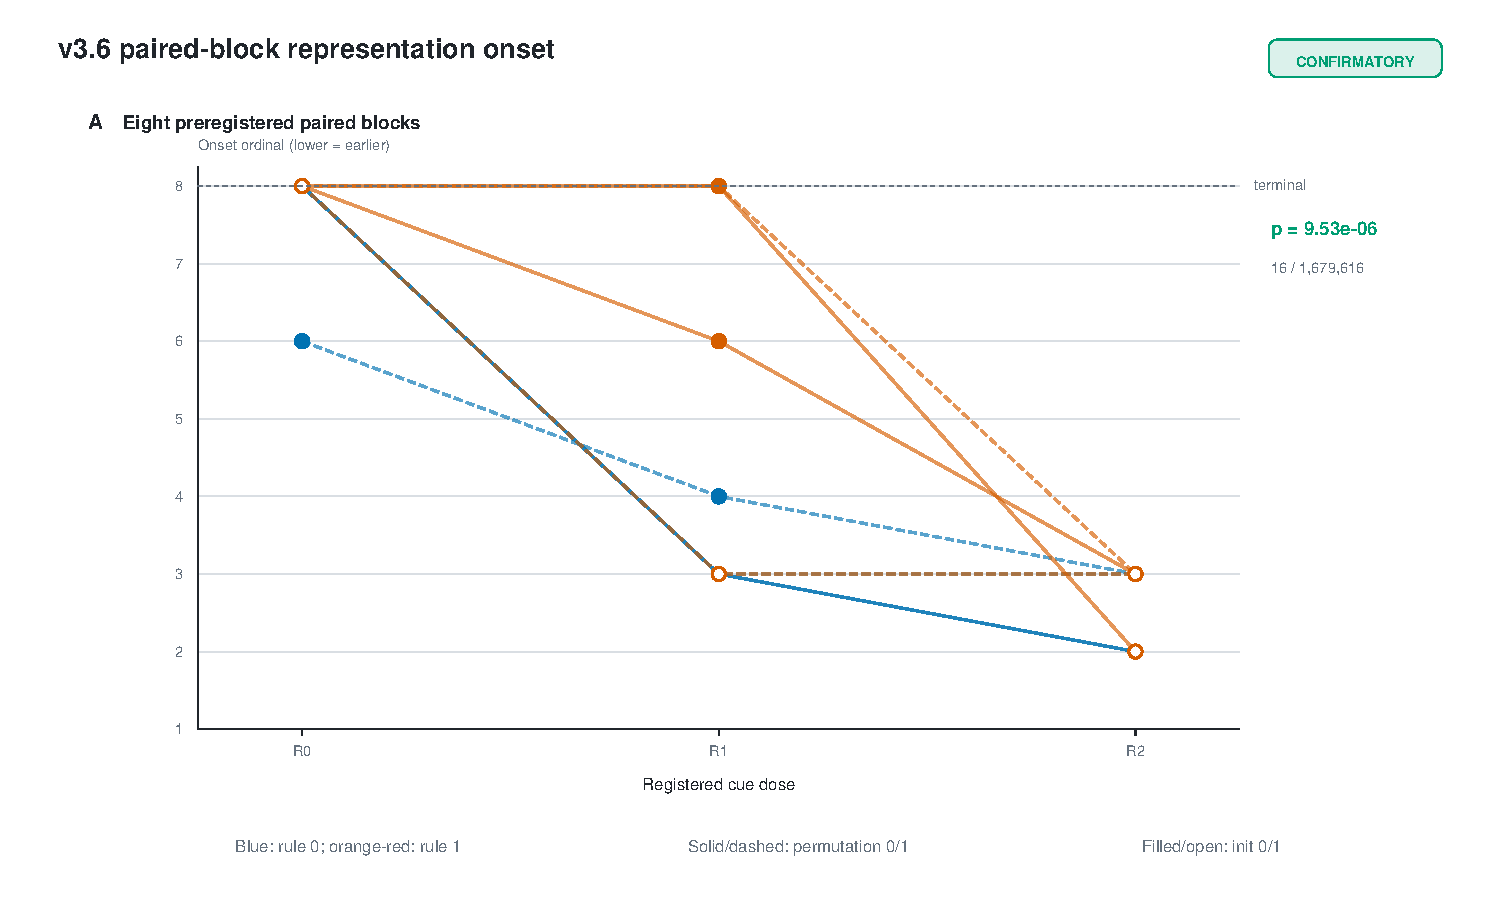
\includegraphics[width=\linewidth]{figures/fig03_v36_paired_onset.pdf}
\caption{Paired terminal-coded onset ordinals for all eight confirmatory
blocks.}
\label{fig:v36-onset}
\end{figure}

\begin{figure}[tb]
\centering
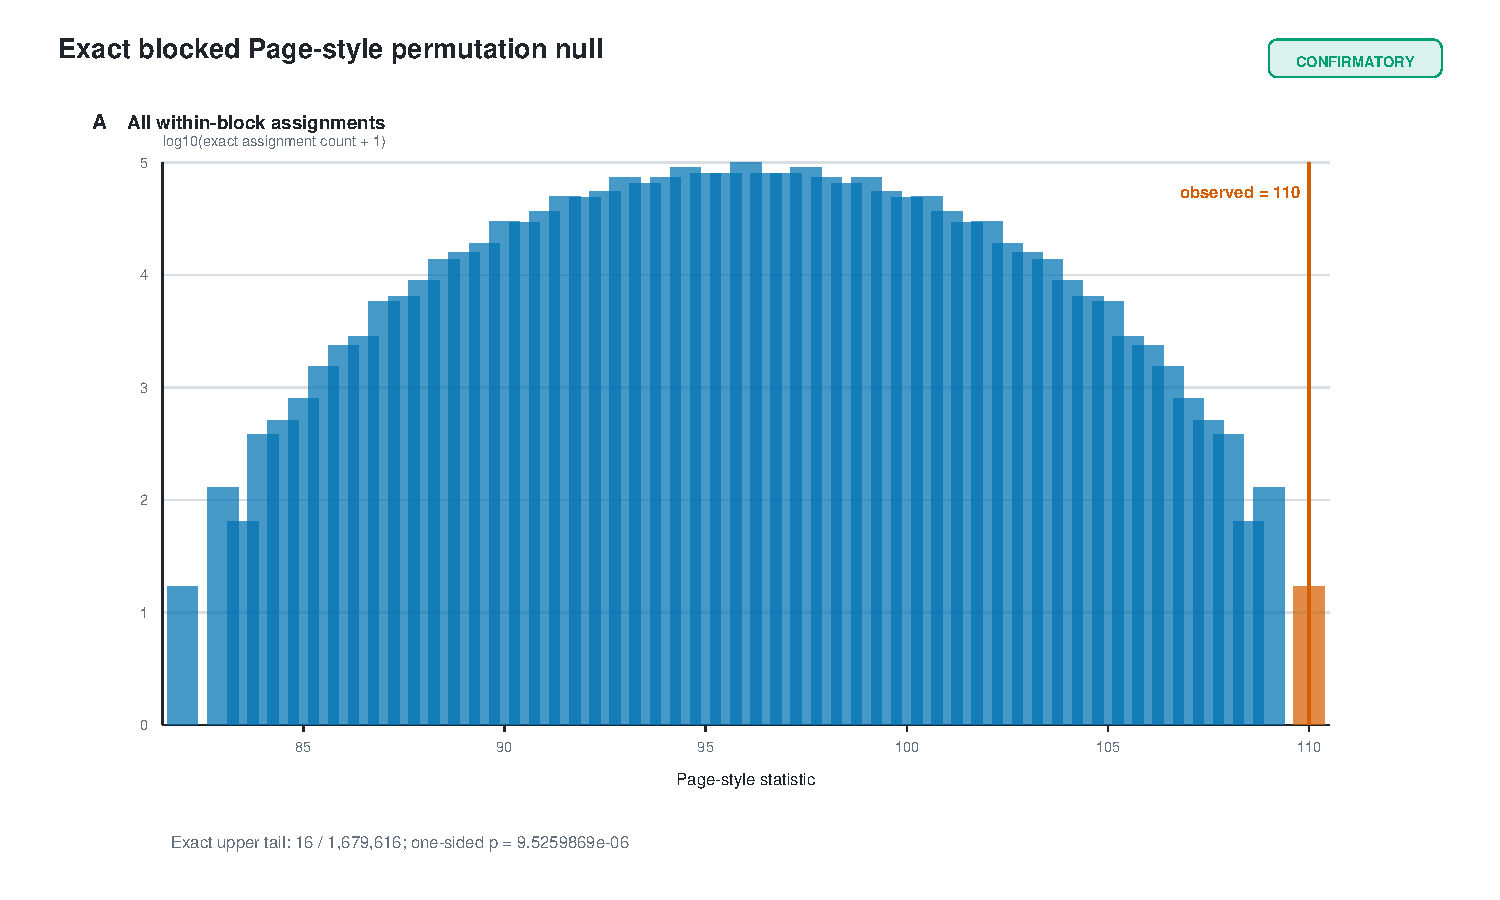
\includegraphics[width=\linewidth]{figures/fig04_v36_exact_null.pdf}
\caption{Exact v3.6 permutation null. Version 3.5 is excluded.}
\label{fig:exact-null}
\end{figure}

\begin{table}[!htbp]
\centering
\caption{Prospectively frozen outcomes across eight paired blocks. Each block crosses one held-out rule, cue permutation, and initialization; trajectories are paired observations, not independent inference units.}
\label{tab:table03-v36-confirmatory-outcomes}
\resizebox{\linewidth}{!}{%
\begin{tabular}{lrrrrrrrrrrr}
\toprule
Version & Status & Condition & n & Onset by 5M & Onset by 10M & Onset exposures (M) & Terminal ordinals & Established by 5M & Established by 10M & Mean R, 5M pre & Mean R, 10M \\
\midrule
v3.6 & confirmatory & R0 & 8 & 0 & 1 & —, —, 7.5, —, —, —, —, — & 8, 8, 6, 8, 8, 8, 8, 8 & 0 & 2 & 1.000239 & 0.432743 \\
v3.6 & confirmatory & R1 & 8 & 5 & 6 & 4, 4, 5, 4, 7.5, —, —, 4 & 3, 3, 4, 3, 6, 8, 8, 3 & 4 & 6 & 0.303076 & 0.110766 \\
v3.6 & confirmatory & R2 & 8 & 8 & 8 & 3, 3, 4, 4, 4, 3, 4, 4 & 2, 2, 3, 3, 3, 2, 3, 3 & 6 & 8 & 0.04371 & 0.005181 \\
\bottomrule
\end{tabular}%
}
\end{table}

\begin{table}[tb]
\centering
\caption{One-sided exact blocked Page-style tests; v3.5 is excluded from every row.}
\label{tab:table04-exact-tests}
\resizebox{\linewidth}{!}{%
\begin{tabular}{lrrrrrrr}
\toprule
Analysis & Blocks & Exact assignments & Observed statistic & Upper-tail count & One-sided p & p<0.05 & v3.5 included \\
\midrule
primary & 8 & 1679616 & 110 & 16 & 9.526e-06 & yes & no \\
rule\_0 & 4 & 1296 & 55.5 & 2 & 0.001543 & yes & no \\
rule\_1 & 4 & 1296 & 54.5 & 8 & 0.006173 & yes & no \\
permutation\_0 & 4 & 1296 & 55.5 & 2 & 0.001543 & yes & no \\
permutation\_1 & 4 & 1296 & 54.5 & 8 & 0.006173 & yes & no \\
\bottomrule
\end{tabular}%
}
\end{table}

\begin{table}[!htbp]
\centering
\caption{Differences are higher registered dose minus lower registered dose within each v3.6 paired block.}
\label{tab:table05-paired-R-differences}
\resizebox{\linewidth}{!}{%
\begin{tabular}{lrrrrrrr}
\toprule
Comparison & Blocks & Mean delta R, 5M & Median delta R, 5M & Mean delta R, 10M & Median delta R, 10M & Mean onset-ordinal delta & Median onset-ordinal delta \\
\midrule
R1\_minus\_R0 & 8 & -0.697162 & -0.789907 & -0.321977 & -0.485173 & -3 & -3.5 \\
R2\_minus\_R0 & 8 & -0.956528 & -0.98357 & -0.427562 & -0.528758 & -5.125 & -5 \\
R2\_minus\_R1 & 8 & -0.259366 & -0.151302 & -0.105585 & -0.001297 & -2.125 & -1 \\
\bottomrule
\end{tabular}%
}
\end{table}

Figures~\ref{fig:v36-onset} and \ref{fig:exact-null} show the paired
onset ordinals and exact null. Tables~\ref{tab:table03-v36-confirmatory-outcomes},
\ref{tab:table04-exact-tests}, and
\ref{tab:table05-paired-R-differences} report confirmatory outcomes, exact
tests, and paired differences. The transition-coding rule is specified in
Supplementary Methods.

\section{Representation persistence after cue removal}
At 5M only the sampler changed for nonzero-cue runs. Zero-step checks verified
unchanged outputs and model, optimizer, scheduler, exposure, and RNG state.
All 13 threshold-positive R1/R2 cells remained positive at 6M
and 10M, supporting learning-path preconditioning rather than a permanently
required shortcut.

\begin{figure}[tb]
\centering
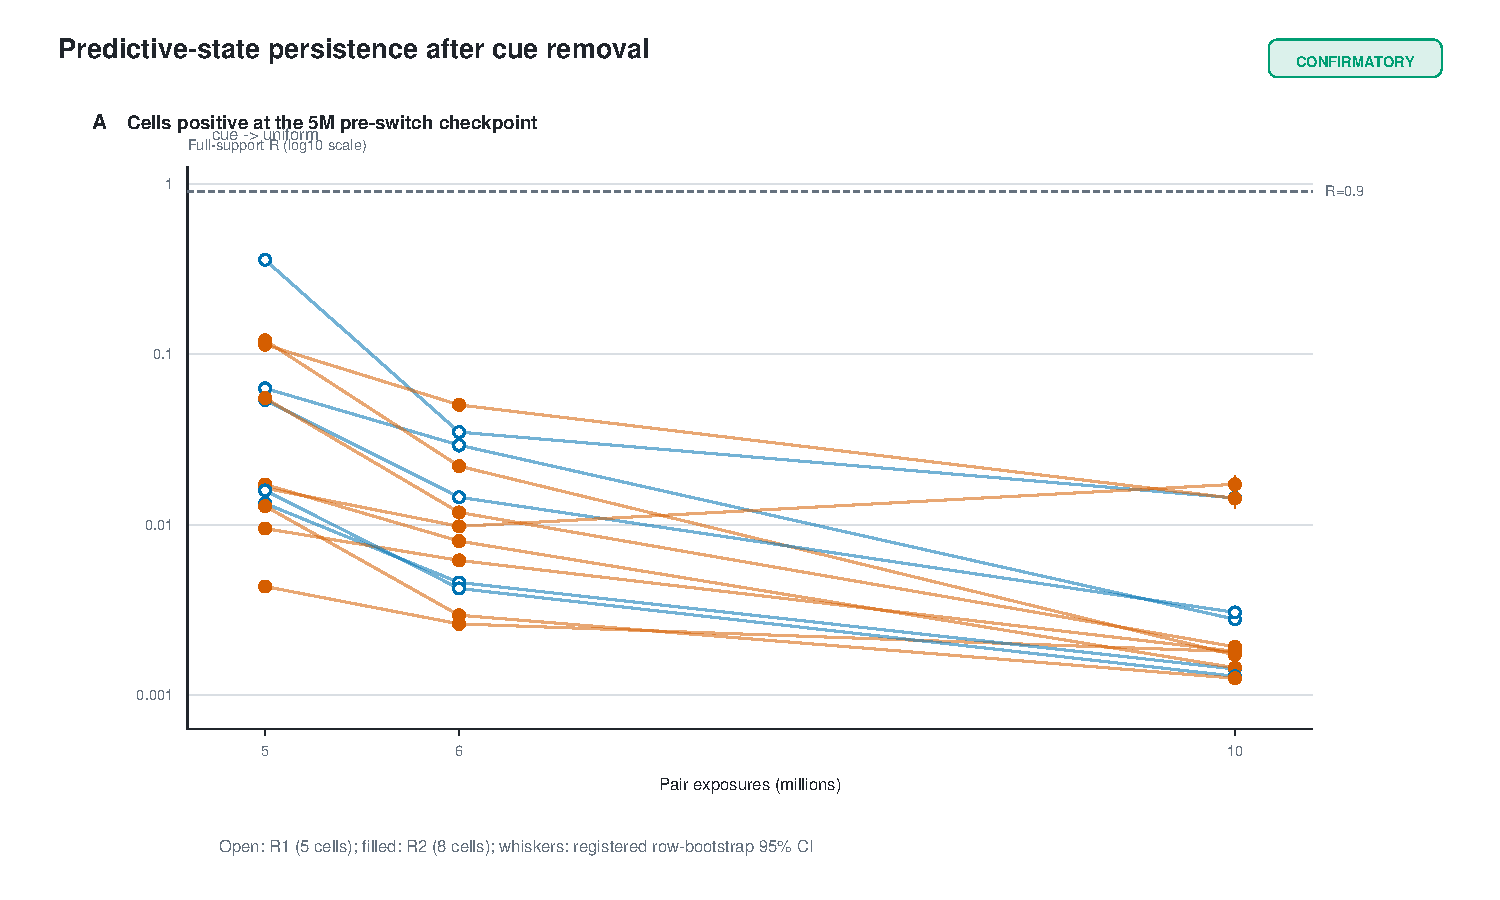
\includegraphics[width=\linewidth]{figures/fig05_v36_persistence.pdf}
\caption{Persistence after return to uniform full support. Whiskers are
registered first-parent-row bootstrap intervals.}
\label{fig:persistence}
\end{figure}

\begin{table}[!htbp]
\centering
\caption{Retention is evaluated only among cells positive at the 5M pre-switch checkpoint.}
\label{tab:table06-cue-removal-persistence}
\resizebox{\linewidth}{!}{%
\begin{tabular}{lrrrrrrrr}
\toprule
Version & Status & Condition & Positive at 5M pre & Retained at 6M & Retained at 10M & Fraction at 6M & Fraction at 10M & Sampler after 5M \\
\midrule
v3.5 & exploratory & C0 & 0 & — & — & — & — & uniform\_full \\
v3.5 & exploratory & C1 & 2 & 2 & 2 & 1 & 1 & uniform\_full \\
v3.5 & exploratory & C2 & 5 & 5 & 5 & 1 & 1 & uniform\_full \\
v3.5 & exploratory & C3 & 5 & 5 & 5 & 1 & 1 & uniform\_full \\
v3.5 & exploratory & geometry\_concentrated & 5 & 5 & 5 & 1 & 1 & uniform\_full \\
v3.5 & exploratory & geometry\_diffuse & 5 & 5 & 5 & 1 & 1 & uniform\_full \\
v3.6 & confirmatory & R0 & 0 & — & — & — & — & uniform\_full \\
v3.6 & confirmatory & R1 & 5 & 5 & 5 & 1 & 1 & uniform\_full \\
v3.6 & confirmatory & R2 & 8 & 8 & 8 & 1 & 1 & uniform\_full \\
\bottomrule
\end{tabular}%
}
\end{table}

Figure~\ref{fig:persistence} and
Table~\ref{tab:table06-cue-removal-persistence} report the persistence
result and zero-step switch audit.

\section{Rule and cue-geometry heterogeneity}
R1 onset occurred in 4/4 rule-0 and 2/4 rule-1
blocks, while R2 onset occurred in 4/4 and 4/4.
The ordered effect spans both rules but the mid-dose response is
rule-dependent. In exploratory matched-index controls, concentrated and
diffuse geometries differed from $m=64$, so equal cue-index values are not
interchangeable.

\begin{figure}[tb]
\centering
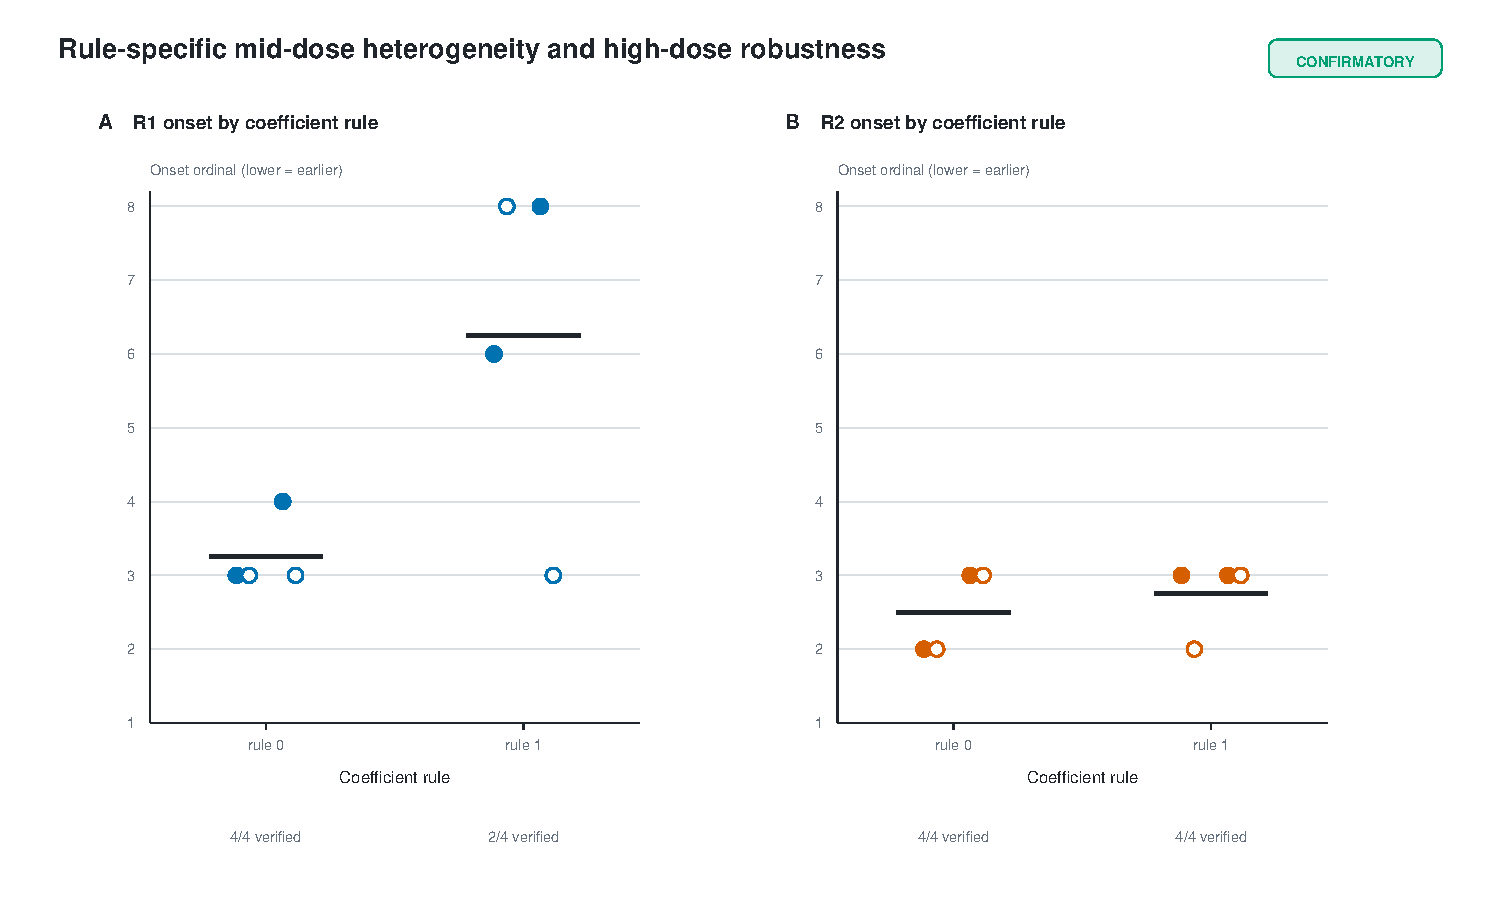
\includegraphics[width=\linewidth]{figures/fig06_v36_rule_heterogeneity.pdf}
\caption{Rule-specific R1 heterogeneity and R2 robustness.}
\label{fig:rule-heterogeneity}
\end{figure}

\begin{figure}[tb]
\centering
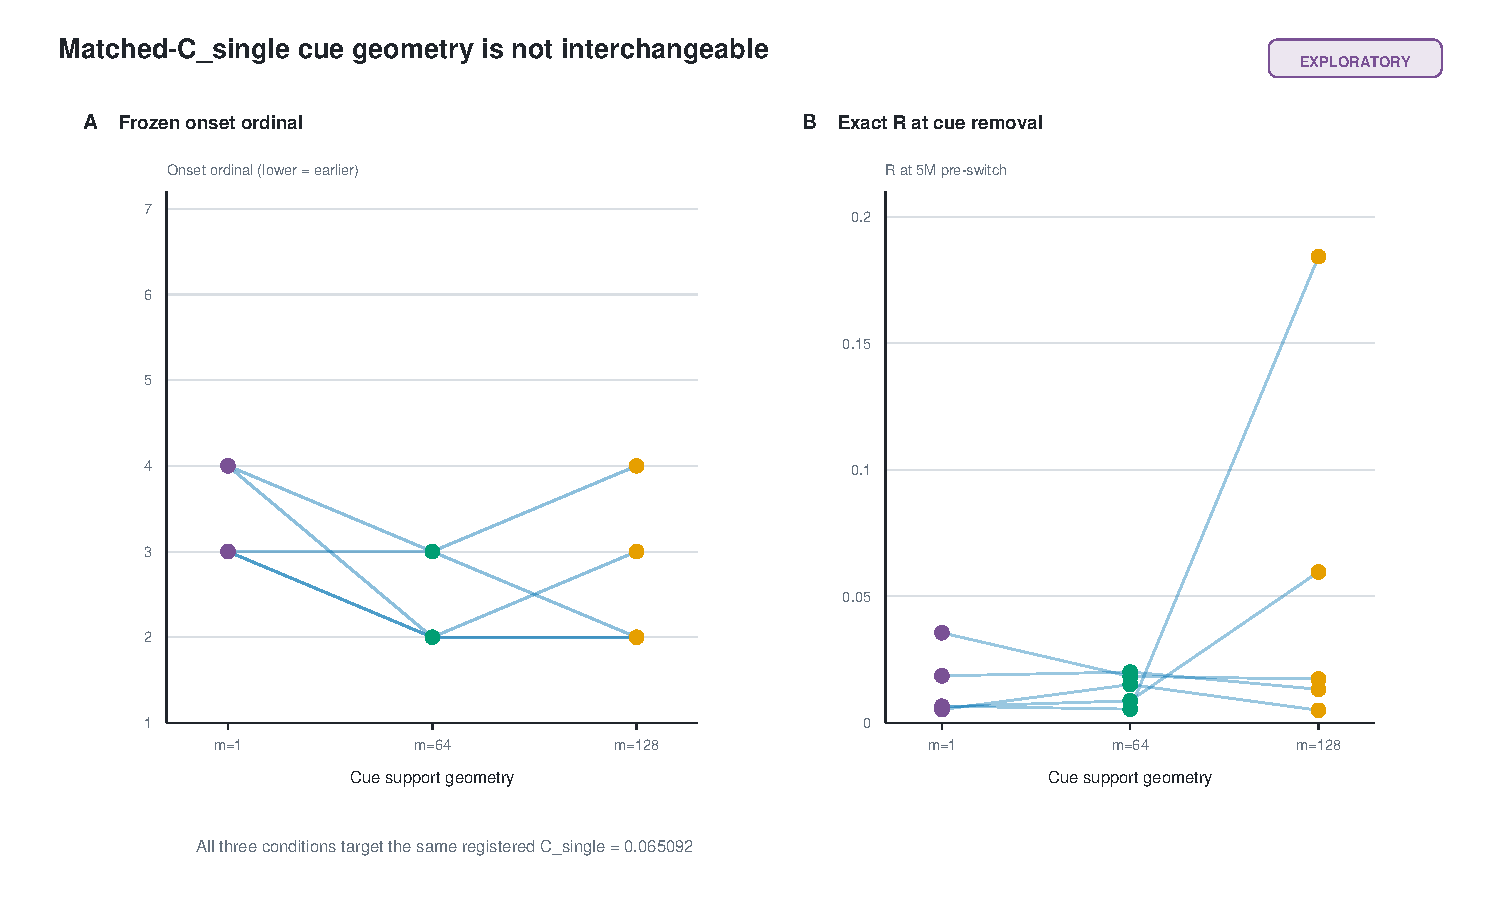
\includegraphics[width=\linewidth]{figures/fig07_v35_geometry_comparison.pdf}
\caption{Exploratory matched-index geometry comparison.}
\label{fig:geometry}
\end{figure}
Figures~\ref{fig:rule-heterogeneity} and \ref{fig:geometry} separate the
confirmatory rule comparison from the exploratory geometry comparison.

\section{Discussion}
Temporary cue-bearing full-support distributions changed whether or when the
frozen Transformer formed the modular predictive center. The target
conditional, marginals, irreducible noise, total pairwise predictable
information, architecture, optimizer, and objective were held fixed.
Persistence after cue removal indicates that the early distribution altered
the learning path rather than supplying a permanently required feature.
Heterogeneity across rules and geometries rejects an explanation based on the
scalar cue index alone.

\subsection{Possible mechanism: symmetry breaking and optimization accessibility}
The evidence suggests a possible optimization-accessibility account: pure
synergy creates a symmetry under which singleton-aligned gradients vanish in
expectation. The parents are individually uninformative, and the symmetric
full-support average cancels their singleton-aligned gradient directions.
Transient cue distributions introduce lower-order statistical
asymmetries while preserving the target conditional and Bayes information
budget. These asymmetries may redirect early optimization toward a state in
which the two parents can be composed; after the task-sufficient
representation forms, the cue is no longer required.

Three observations are consistent with this account: onset was ordered by
registered cue dose, threshold-positive representations persisted after cue
removal, and the frozen gradient audits showed changes in gradient coherence
around observed transitions. This is mechanistic interpretation, not a causal
mediation result. \emph{Gradient statistics are correlates of transition
dynamics, not identified causal mediators.} The data do not establish a
universal loss-landscape mechanism or a unique circuit.

\subsection{Practical implication: distributional bootstrapping}
The result suggests a possible design principle: temporary training
distributions can be used to improve access to otherwise hard-to-reach
compositional representations when the final task distribution contains
high-order dependencies. This is a hypothesis for bounded, auditable
interventions, not a claim that all AI training should use low-order cues.

\section{Limitations}
First, model scale is limited to one approximately 2M-parameter Transformer
family; scale dependence remains open. Second, the parent-exposed interface
intentionally controls variable identification; recurrent context discovery
and variable selection remain future work. Third, exact soft-label training
isolates representation formation from sampled-label variance; sampled-token
training remains future work. Fourth, finite-field modular arithmetic is a
controlled model organism rather than a proxy for the full range of
natural-data learning. Fifth, the experiments identify a distribution
intervention but do not establish a universal loss-landscape mechanism.

The study also uses one field size, one noise level, a finite checkpoint grid,
and eight confirmatory blocks. The exact test is valid for the frozen
randomization structure but does not make the tested rules a population sample
of all modular tasks. The result is not a universal Transformer claim, not a
thermodynamic phase transition, and not evidence that the recurrent production
task is solved. These results are excluded from the original scaling fit.

\section{Reproducibility statement}
The final result is tagged \texttt{kepler-v3.6-confirm1}. Frozen hashes,
environment, test definitions, counts, and provenance are indexed in the
package. The lightweight verifier recomputes distribution audits, transition
coding, all 1,679,616 exact assignments, figures,
and tables without optimizer steps.

\begin{table}[!htbp]
\centering
\caption{Counts and integrity flags are read from the frozen result and confirmatory freeze records.}
\label{tab:table07-protocol-integrity}
\resizebox{\linewidth}{!}{%
\begin{tabular}{lrrrrrrrrrrrrr}
\toprule
Version & Status & Registered runs & Completed runs & Checkpoints & Sidecars valid & Evaluations & Probe reports & Gradient audits & Switch checks & Switches passed & Max exposure & Objective & Excluded from scaling fit \\
\midrule
v3.5 & exploratory & 30 & 30 & 330 & yes & 360 & 210 & 150 & 30 & yes & 10000000 & exact\_soft\_label\_cross\_entropy & yes \\
v3.6 & confirmatory & 24 & 24 & 264 & yes & 288 & 168 & 0 & 24 & yes & 10000000 & exact\_soft\_label\_cross\_entropy & yes \\
\bottomrule
\end{tabular}%
}
\end{table}

\begin{table}[!htbp]
\centering
\caption{The manuscript uses the allowed scoped statements and excludes the listed overclaims.}
\label{tab:table08-claim-boundaries}
\resizebox{\linewidth}{!}{%
\begin{tabular}{lrr}
\toprule
Topic & Allowed statement & Excluded statement \\
\midrule
Causal scope & The registered transient cue-bearing full-support distributions changed onset timing or probability in the frozen parent-exposed task and model family. & Singleton mutual information alone is the causal variable. \\
Persistence & Threshold-positive representations persisted after return to uniform full support. & The cue is permanently required for prediction. \\
Generality & The ordered effect replicated across the two new rules and two new permutations tested. & This is a universal Transformer property. \\
Dynamics & The registered checkpoints show abrupt or delayed representation formation in some trajectories. & The result is a thermodynamic phase transition. \\
Recurrent task & The parent-exposed task isolates a mechanism relevant to the broader program. & The recurrent production task has been solved. \\
Scaling & The experiments are mechanism-focused exploratory and confirmatory audits. & The result belongs in the original scaling fit. \\
C\_single & C\_single is a registered scalar cue index used to order selected distributions. & C\_single is a unique-information percentage. \\
\bottomrule
\end{tabular}%
}
\end{table}

Tables~\ref{tab:table07-protocol-integrity} and
\ref{tab:table08-claim-boundaries} summarize protocol integrity and claim
boundaries.

\section{Data and code availability}
Code, manifests, result JSON, source data, and verification scripts are
included in the repository. Checkpoints are referenced by SHA-256 sidecars and
are unnecessary for lightweight verification.

\section{Supplementary methods}
\subsection{Task objective, evaluation, and probes}
Exact soft-label cross-entropy was used throughout the parent-exposed
experiments: at each observed pair, the target was the analytic noisy
conditional rather than one sampled label. Evaluation enumerated all
66,049 ordered parent pairs. Every checkpoint recorded exact conditional KL,
normalized $R$, center accuracy, center probability, predictive entropy, and a
2,000-replicate first-parent-row bootstrap interval. Selected checkpoints
included layer-wise linear, fixed-Fourier, and fixed-capacity MLP probes.

\subsection{Cue-family construction and audit}
Frozen cue permutations and coefficients reweighted the complete pair space
while preserving strictly positive probability for every pair. Lambda was
solved by deterministic root finding for each preregistered target, not
selected from model outcomes. Exhaustive enumeration verified marginal
uniformity, conditional invariance, joint information, and full support.

\subsection{Model and optimization}
The manifest records 2,045,568 core
parameters, width 168, batch size
4,096, exact soft-label cross-entropy, AdamW
learning rate $3\times10^{-4}$,
betas
$(0.9,0.95)$, weight decay
0.1, clipping at 1.0,
5M warmup exposures, and an
absolute-exposure cosine schedule.

\subsection{Transition coding}
Probe checkpoints were 2M, 3M, 4M, 5M, 6M, 7.5M, and 10M. Onset required
$R<0.9$ and layer-6 linear accuracy above 0.5, retained at the next checkpoint.
Establishment required $R<0.1$, center accuracy above 0.9, and layer-6 linear
accuracy above 0.9.

\subsection{Exact test}
Within-block terminal onset ordinals were converted to doubled midranks, with
earlier onset ranked higher. All six label assignments were combined across
eight blocks, giving $6^8=1,679,616$ assignments.

\subsection{Artifact integrity}
The freeze records every tag, manifest and result hash, the environment lock,
test definition and result, and artifact counts. This manuscript revision
changes only the \texttt{paper/} tree; no prior scientific artifact changes.

\begin{thebibliography}{9}
\bibitem{power2022grokking}
A. Power, Y. Burda, H. Edwards, I. Babuschkin, and V. Misra.
\newblock Grokking: Generalization beyond overfitting on small algorithmic
datasets.
\newblock \emph{arXiv:2201.02177}, 2022.
\newblock \url{https://arxiv.org/abs/2201.02177}.

\bibitem{nanda2023progress}
N. Nanda, L. Chan, T. Lieberum, J. Smith, and J. Steinhardt.
\newblock Progress measures for grokking via mechanistic interpretability.
\newblock \emph{arXiv:2301.05217}, 2023.
\newblock \url{https://arxiv.org/abs/2301.05217}.

\bibitem{bengio2009curriculum}
Y. Bengio, J. Louradour, R. Collobert, and J. Weston.
\newblock Curriculum learning.
\newblock In \emph{Proceedings of the 26th International Conference on
Machine Learning}, 2009.
\newblock \url{https://icml.cc/2009/papers/119.pdf}.

\bibitem{williams2010pid}
P. L. Williams and R. D. Beer.
\newblock Nonnegative decomposition of multivariate information.
\newblock \emph{arXiv:1004.2515}, 2010.
\newblock \url{https://arxiv.org/abs/1004.2515}.
\end{thebibliography}

\end{document}
